\setchapterpreamble[u]{
    \dictum[Leonard Nimoy como Mr. Spock en \textit{Start Trek TOS}]{\textquote{Computers make excellent and efficient servants, but I have no wish to serve under them.}}
}
\chapter{RISC-V}

% RISC-V es una arquitectura de estándar abierto que sigue los principios de las arquitecturas RISC (\textit{Reduced Instruction Set Computers} o Computadoras de Conjunto Reducido de Instrucciones), de tipo load-store y conjunto de instrucciones variable y modular, y 32 registros de propósito general% (el registro cero está conectado a tierra)\footnote{También existe un subconjunto para procesadores embebidos de 16 registros}.

% RISC-V es tan solo un ISA (Instruction Set Architecture), es decir, una definición de un conjunto de instrucciones que debe soportar cualquier procesador que quiera ejecutar software compatible con dicha arquitectura.
RISC-V es tan solo un ISA (\textit{Instrucion Set Architecture}), es decir, la parte del procesador que debe tener en cuenta el compilador o el programador para generar software ejecutable por una máquina de esa arquitectura \cite{HenessyPattersonCAQA}. La principal diferencia con otras ISAs como MIPS, ARM o x86 es que RISC-V es una arquitectura de estándar abierto y gratuito, por lo que cualquiera puede diseñar su propio procesador que la implemente. 
% A diferencia de AMD, Intel o ARM, \mbox{RISC-V} International no fabrica ningún tipo de procesador; en su lugar diversas compañías y organizaciones crean sus propias implementaciones \cite{RiscVExchangeCores}, con distintas características. 

La arquitectura RISC-V tiene un conjunto de instrucciones \textit{reducido} o RISC (\textit{Reduced Instruction Set Computer}), por lo que cuenta con menos instrucciones que una arquitectura compleja o CISC (\textit{Complex Instruction Set Computer}). Al contrario que en CISC, las instrucciones en RISC son más simples y cada una de ellas realiza una sola función muy concreta. Asimismo, decimos que RISC-V es una arquitectura \textit{load/store}, también llamada de \textit{registro a registro}, en la que el procesador cuenta con un \textit{banco de registros} en el que se realizan las operaciones, y nunca directamente sobre la memoria. Es decir, para ejecutar un cálculo usando datos de la memoria primero es necesario usar instrucciones de \textit{load} para llevar los operandos a los registros, luego realizar el cálculo con todas las instrucciones aritmético-lógicas necesarias y, finalmente, usar un \textit{store} para desplazar el resultado de nuevo a la memoria.

 La arquitectura RISC-V es modular, existiendo distintos conjuntos base, y extensiones que pueden añadir funcionalidades a un procesador. Para que un procesador soporte la arquitectura RISC-V no privilegiada debe implementar el conjunto base \textbf{I} de 32, 64 o 128 bits; aunque puede usarse el conjunto base \textbf{E} de 32 bits para sistemas embebidos, que cuenta con la mitad de registros accesibles \cite{RiscVSpec1}. Asimismo, se definen múltiples extensiones que pueden soportarse en cada implementación. A continuación se listan las extensiones no privilegiadas ratificadas en la versión 20191213 del ISA:

\begin{itemize}[noitemsep]
    \item[\textbf{M}] Multiplicación y división entera
    \item[\textbf{A}] Instrucciones atómicas
    \item[\textbf{F}] Coma flotante de precisión sencilla (IEEE-754)
    \item[\textbf{D}] Coma flotante de precisión doble (IEEE-754)
    \item[\textbf{Q}] Coma flotante de precisión cuádruple
    \item[\textbf{C}] Instrucciones comprimidas (como el conjunto \textit{Thumb} de ARM)
    \item[\textbf{Zicsr}] CSR: Registro de Control y Estado
    \item[\textbf{Zifencei}] Barrera o \textit{fence} para la fase \textit{fetch} de instrucciones
\end{itemize}

También cuenta con extensiones aún no ratificadas para manipulación de bits, SIMD (\textit{Single Instruction Multiple Data}), operaciones vectoriales, criptografía, JIT (aceleración de lenguajes intepretados), virtualización... Parte del espacio de instrucciones está reservado para la implementación de conjuntos de instrucciones propietarios.

% \begin{recuadro}
Para identificar las características de la arquitectura de un procesador, suele usarse como nomenclatura el prefijo \textit{RV}, seguido del número de bits y los subconjuntos de instrucciones que soporta (comenzando con la ISA base). Por ejemplo, un procesador de propósito general de 64 bits con multiplicación y división de enteros, instrucciones atómicas y coma flotante sería un procesador RV64IMAFD; mientras que un procesador embebido con la extensión criptográfica sería un RV32EK.

En ocasiones nos referiremos a la extensión \textbf{G}, que es una abreviatura de \textbf{IMAFDZicsrZifencei} y comprende todos los conjuntos necesarios para implementar un procesador de propósito general. Por lo tanto, un procesador RV32/64G es un objetivo estable para el desarrollo de software, pues todas sus extensiones están ratificadas.
% \end{recuadro}

% En caso de querer implementar un dispositivo embebido, es posible usar como conjunto base el subconjunto \textbf{E} en lugar de \textbf{I}, que solo tiene acceso a 16 de los 32 registros entre otras muchas limitaciones.

% \section{Formato de las instrucciones}

El formato de las instrucciones es el siguiente:

\begin{figure}[h]
\begin{center}
\setlength{\tabcolsep}{4pt}
\begin{tabular}{p{0.3in}@{}p{0.8in}@{}p{0.6in}@{}p{0.18in}@{}p{0.7in}@{}p{0.6in}@{}p{0.6in}@{}p{0.3in}@{}p{0.5in}l}
\\
\multicolumn{1}{c}{\instbit{31}} &
\instbitrange{30}{25} &
\instbitrange{24}{21} &
\multicolumn{1}{c}{\instbit{20}} &
\instbitrange{19}{15} &
\instbitrange{14}{12} &
\instbitrange{11}{8} &
\multicolumn{1}{c}{\instbit{7}} &
\instbitrange{6}{0} \\
\cline{1-9}
\multicolumn{2}{|c|}{funct7} &
\multicolumn{2}{c|}{rs2} &
\multicolumn{1}{c|}{rs1} &
\multicolumn{1}{c|}{funct3} &
\multicolumn{2}{c|}{rd} &
\multicolumn{1}{c|}{opcode} &
R-type \\
\cline{1-9}
\\
\cline{1-9}
\multicolumn{4}{|c|}{imm[11:0]} &
\multicolumn{1}{c|}{rs1} &
\multicolumn{1}{c|}{funct3} &
\multicolumn{2}{c|}{rd} &
\multicolumn{1}{c|}{opcode} &
I-type \\
\cline{1-9}
\\
\cline{1-9}
\multicolumn{2}{|c|}{imm[11:5]} &
\multicolumn{2}{c|}{rs2} &
\multicolumn{1}{c|}{rs1} &
\multicolumn{1}{c|}{funct3} &
\multicolumn{2}{c|}{imm[4:0]} &
\multicolumn{1}{c|}{opcode} &
S-type \\
\cline{1-9}
\\
\cline{1-9}
\multicolumn{1}{|c|}{imm[12]} &
\multicolumn{1}{c|}{imm[10:5]} &
\multicolumn{2}{c|}{rs2} &
\multicolumn{1}{c|}{rs1} &
\multicolumn{1}{c|}{funct3} &
\multicolumn{1}{c|}{imm[4:1]} &
\multicolumn{1}{c|}{imm[11]} &
\multicolumn{1}{c|}{opcode} &
B-type \\
\cline{1-9}
\\
\cline{1-9}
\multicolumn{6}{|c|}{imm[31:12]} &
\multicolumn{2}{c|}{rd} &
\multicolumn{1}{c|}{opcode} &
U-type \\
\cline{1-9}
\\
\cline{1-9}
\multicolumn{1}{|c|}{imm[20]} &
\multicolumn{2}{c|}{imm[10:1]} &
\multicolumn{1}{c|}{imm[11]} &
\multicolumn{2}{c|}{imm[19:12]} &
\multicolumn{2}{c|}{rd} &
\multicolumn{1}{c|}{opcode} &
J-type \\
\cline{1-9}
\end{tabular}
\end{center}
\caption[Formato de instrucciones base en RISC-V 32 bits]{Formato de instrucciones base de 32 bits. Cada subcampo del inmmediato se describe con la posición de los bits (imm[{\em x}\,]) relativa al subcampo, y no a la instrucción como suele hacerse. Extraído de \cite{RiscVSpec1} }
\label{fig:baseinstformats}
\end{figure}

% En el capítulo \ref{ch:desCore} de la página \pageref{ch:desCore} se exponen distintas implementaciones RV32/64 y la elegida para incluir el diseño de la NoC.

La codificación de las instrucciones es fija, y podemos distinguir los siguientes seis formatos en el conjunto base~\cite{BerkeleyCS61C7}:

\begin{itemize}[noitemsep]
    \item [\textbf{R}] Instrucciones en las que se especifican 3 registros: 2 que almacenan los operandos fuente y un destino en el que guardar el resultado. Para poder realizar más operaciones, este tipo de instrucciones cuentan con bits extra para seleccionar la operación a realizar.
    \item [\textbf{I}] Instrucciones que incluyen un operando \textit{inmediato} (fijo en la codificación de la instrucción), además de otro registro fuente y un destino.
    \item [\textbf{S}] Instrucciones de \textit{store}, encargadas de guardar los datos de un registro a la memoria.
    \item [\textbf{SB}] Instrucciones de ramificación \textit{branch}, que implementan saltos condicionales.
    \item [\textbf{U}] Instrucciones en las que se especifica un registro destino y un inmediato (de 20 bits, más largo que en las de tipo I).
    \item [\textbf{UJ}] Instrucciones de salto incondicional.
\end{itemize}

\section{Elección del núcleo RISC-V}
\label{sec:desCore}

Para seleccionar el núcleo (\textit{core}) a modificar, se ha explorado la lista de \textit{cores} de RISC-V Exchange \cite{RiscVExchangeCores}. El objetivo principal ha sido buscar un proyecto en el que fuese sencillo embeber una NoC como prueba de concepto, sin importar mucho las características técnicas del procesador, su potencia o sus resultados en \textit{benchmarks}. Por lo tanto, hemos priorizado que su lenguaje de programación fuese conocido, tuviese licencias abiertas, y una amplia documentación y herramientas de desarrollo.

Se ha filtrado la selección buscando Cores escritos en lenguajes conocidos (VHDL o SystemVerilog) y con licencia libre reconocida por OSI (Apache, BSD, GPL o MIT) \cite{OSILicenses}. Finalmente, la selección se redujo a los siguientes núcleos:

\begin{description}
    \item[SweRV Core EH1] [RV32IMCZ]: Es superescalar con 2 vías de lanzamiento (dual issue) y segmentación en 9 fases. Ha sido fabricado en tecnología de 28nm, pero cuenta con optimizaciones para FPGA. Creado por Western Digital. Tiene 4 unidades aritmético-lógicas (ALU), 2 \textit{early} y 2 \textit{late}, cada una conectada a una de las vías del ILP \cite{RepoSwervEH1}.
    \item[SweRV Core EH2] [RV32IMACZ]: Basado en el EH1, se le añade multithreading para 2 hilos, y por lo tanto también se le agregan instrucciones atómicas \cite{RepoSwervEH2}.
    \item [SweRV Core EL2] [RV32IMC]: Es un núcleo mucho más sencillo que el EH1 creado para reemplazar a las máquinas de estados y otras funciones lógicas implementadas en Sistema en Chip (haciendo que puedan ser actualizadas). La segmentación es en solo 4 etapas y es escalar \cite{RepoSwervEL2}.
    \item [biRISC-V] [RV32IMZicsr]: Superescalar con dual issue y segmentación en 6-7 etapas, tiene un divisor hardware, 1 unidad de load-store y 2 ALUs. Implementa también instrucciones privilegiadas, por lo que puede ejecutar sistemas operativos de propósito general \cite{RepoBiRISCV}.
    \item [PicoRV32] [RV32IMC]: Es un pequeño procesador de menos de 2000 LUTs, por lo que caben múltiples en una FPGA. % Una idea alternativa hubiese sido crear una interfaz de red para este procesador, y conectar varios de ellos en una FPGA formando un SoC manycore \cite{PicoRV32gh}.
\end{description}

Algunos otros núcleos y herramientas que se consideraron y fueron descartados en fases tempranas (principalmente por el lenguaje de programación o su complejidad) fueron los siguientes:

\begin{description}
    \item [WARP-V] Está escrito en TL-Verilog y es un generador de cores con muchas opciones de configuración. Parte de este trabajo podría haber sido añadir al WARP-V la opción de usar una NoC, al igual que existen opciones para añadir o quitar etapas del pipeline.
    \item [Rocket Chip] Más que un procesador, se trata de un generador escrito en \textbf{Chisel}, lenguaje libre de definición de hardware basado en Scala que emite código sintetizable en Verilog. Ha sido diseñado por el departamento de D. Patterson, A. Waterman y K. Asanović, creadores del RISC-V. \cite{AsanovicRocketChip}.
    \item [BOOM] [RV64GC] \textit{Berkeley Out-of-Order Machine}. Está creado por el mismo departamento que Rocket y con herramientas muy similares. Su característica principal es su alto grado de paralelismo a nivel de instrucción. Sin embargo, su estructura es mucho más compleja y, por lo tanto, difícil de modificar \cite{Celio:EECS-2015-167}.
\end{description}

La principal ventaja de Rocket y BOOM es que, debido a su longevidad y soporte a lo largo del tiempo, cuentan con amplia documentación, literatura, herramientas, y han sido implementados tanto en FPGA como en ASICs, por lo que aunque no han sido usados directamente en este proyecto, sí que se ha consultado en ocasiones literatura relacionada con estos procesadores.

\begin{figure}[h]
    \centering
    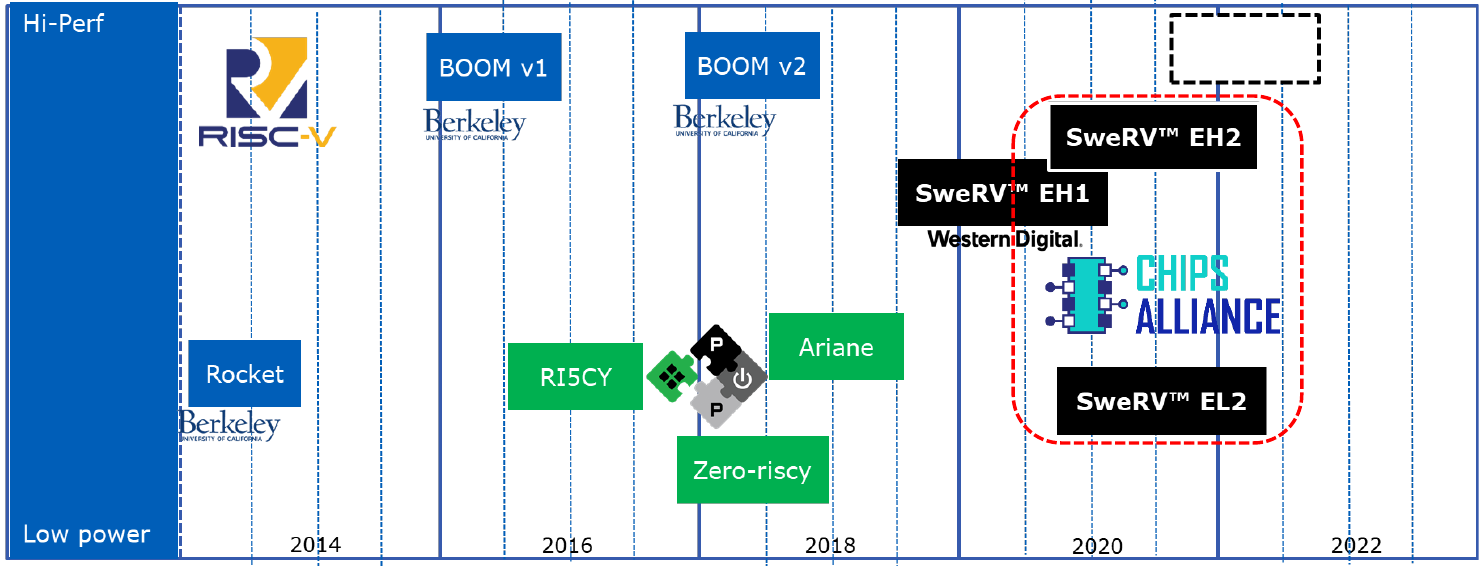
\includegraphics[width=\linewidth]{images/external/roadmap_compare.png}
    \caption[Comparativa de la potencia de varios Cores RISC-V de código abierto]{Comparativa de la potencia de varios Cores RISC-V de código abierto. Resaltado en rojo los procesadores de la familia SweRV. Extraído de \citetitle{SweRVRoadmap}~\cite{SweRVRoadmap}.}
    \label{fig:swerv_comparative}
\end{figure}

Finalmente, se eligió la familia SweRV debido a la familiaridad con el proyecto (se usa este procesador en la actividad formativa ``Implementación ASIC de 28nm del procesador RISC V"). En la figura \ref{fig:swerv_comparative} se muestra una comparativa de dichos procesadores con otros cores de código abierto. Dentro de los procesadores de esta familia, se decidió modificar el EL2 por su sencillez y los pocos recursos humanos de los que se dispone en este proyecto. No obstante, tratándose de una prueba de concepto, siempre es posible en el futuro aplicar las técnicas aprendidas a otros productos más complejos, con mejoras y optimizaciones.

\setchapterpreamble[u]{
    \dictum[Bob Kahn en \textit{Where Wizards Stay Up Late}]{\textquote{It’s one thing when you plug in to a socket in the wall and electrons flow. It’s another thing when you have to figure out, for every electron, which direction it takes.}}
}
\chapter{Resultados de la síntesis del SweRV-EL2 y NoC}

Aunque el objetivo principal del proyecto es realizar un diseño RTL, se ha sintetizado dicho diseño para la plataforma objetivo Virtex-7 VC707 Evaluation Kit, que hace uso de una FPGA Virtex-7 XC7VX485T-2FFG1761C \cite{XilinxVC707}.

Esta FPGA cuenta con 700 pines de entrada/salida, más de 300 mil LUTs y 600 mil registros.

\section{Área utilizada por el diseño}
Se ha generado un reporte de utilización usando Xilinx Vivado tras sintetizar para la Virtex-7 con la configuración por defecto. Debido a que aún no se ha realizado la fase de implementación ni sus optimizaciones, estos resultados son una mera estimación, pudiendo ser diferentes al realizar el flujo de implementación a la FPGA.

En total, el diseño sintetizado (que incluye \textit{core}, memoria e interfaz DMI) ocupa un $14\%$ de las LUTs de la FPGA (40 mil), y un $4\%$ de sus registros (23 mil), siendo con diferencia el \textit{core} el que más área consume: un $12\%$ y $3.59\%$ de los recursos disponibles en la FPGA respectivamente (36 mil y 21 mil).

Dentro del \textit{core}, su elemento más pesado es la IFU, con 11 mil LUTs ($3.69\%$), seguido de la EXU con 10 mil LUTs ($3.18\%$). Por lo tanto, solo estos dos elementos ya forman el 40\% de los LUTs consumidos por el core, dejando un $3.77\%$ del total (11 mil LUTs) para el DEC y el LSU. Por otra parte, dos tercios de los registros del \textit{core} son utilizados por el IFU. En la figura \ref{fig:plots_area_core} se visualizan dichos áreas. Todos los \textit{senders} y \textit{receivers} instanciados a este nivel (es decir, sin contar los de dentro de los wrappers) sumados hacen uso de 66 LUTs y 79 flip-flops, siendo los receptores los que más registros consumen (70 de los 79), puesto que deben almacenar los datos del paquete recibido. El detector de reloj ha sido sintetizado a un flip-flop.
\begin{figure}[h]
    \centering
    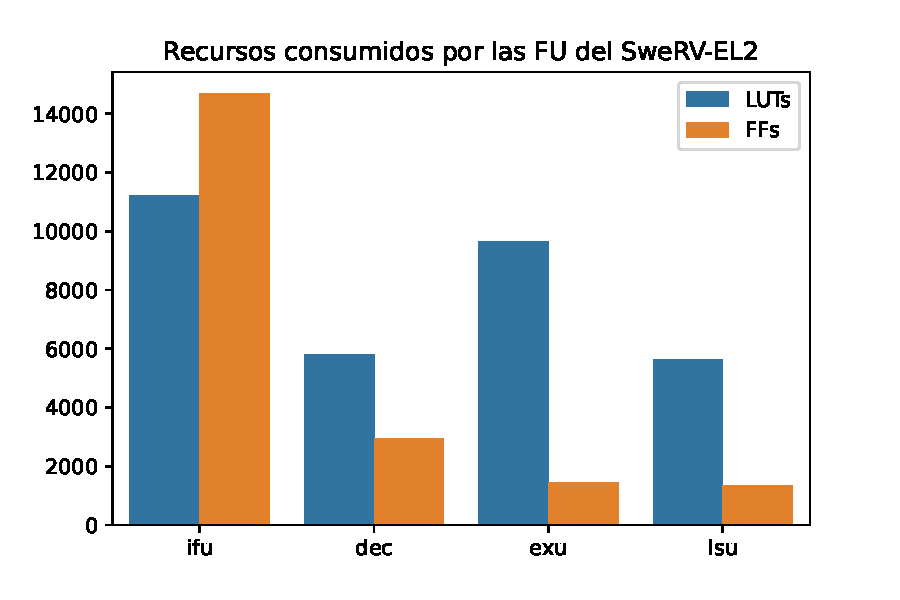
\includegraphics[width=12cm]{images/plots/swerv_fu.pdf}
    \caption[Recursos consumidos por las unidades funcionales del \textit{core}.]{Recursos consumidos por las unidades funcionales del \textit{core}.}
    \label{fig:plots_area_core}
\end{figure}

\subsection{Recursos utilizados en la unidad de ejecución y la NoC}
A continuación analizaremos el uso de recursos de la EXU, a la que se le ha incluido una NoC. 
En la figura \ref{fig:plots_area_exu} se visualizan los datos mencionados a continuación.
De los 9700 LUTs usados por la EXU, 2700 ($28\%$) son ocupados por los encaminadores y conexiones de la NoC. A los wrappers del multiplicador y el divisor se les asignan 1433 y 744 LUTs respectivamente. Otra gran parte de los recursos de la EXU (2214 LUTs, $23\%$) son asignados al módulo \textit{i\_x\_ff}, encargado de parte de la lógica de predicción de salto.

\begin{figure}[p]
    \centering
    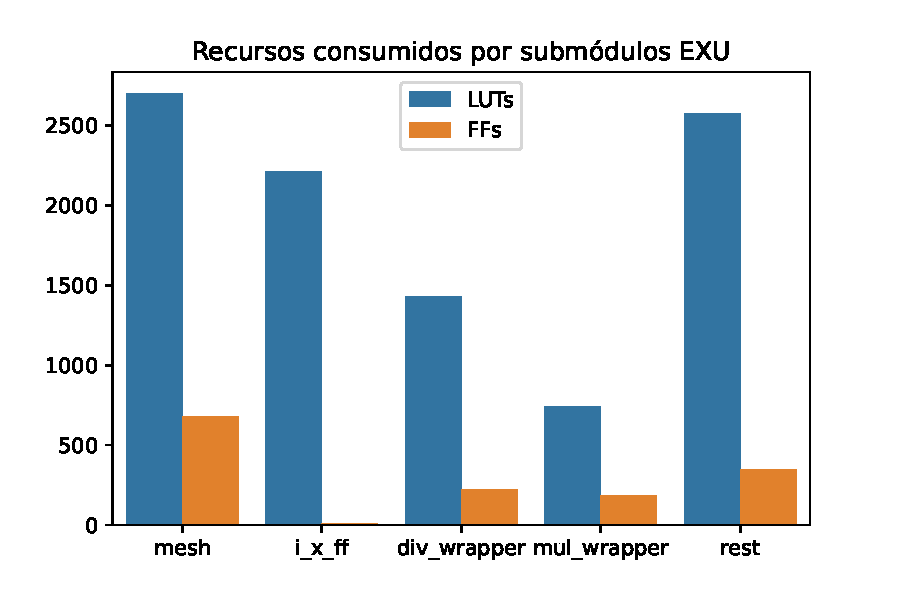
\includegraphics[width=13cm]{images/plots/swerv_exu.pdf}
    \caption[Recursos consumidos por los submódulos de la unidad de ejecución.]{Recursos consumidos por los submódulos de la unidad de ejecución. En rest se muestran los LUTs y \textit{flip-flops} utilizados tanto para el resto de submódulos de la EXU como para la lógica y conexiones del módulo EXU.}
    \label{fig:plots_area_exu}
\end{figure}

\begin{figure}[p]
    \centering
    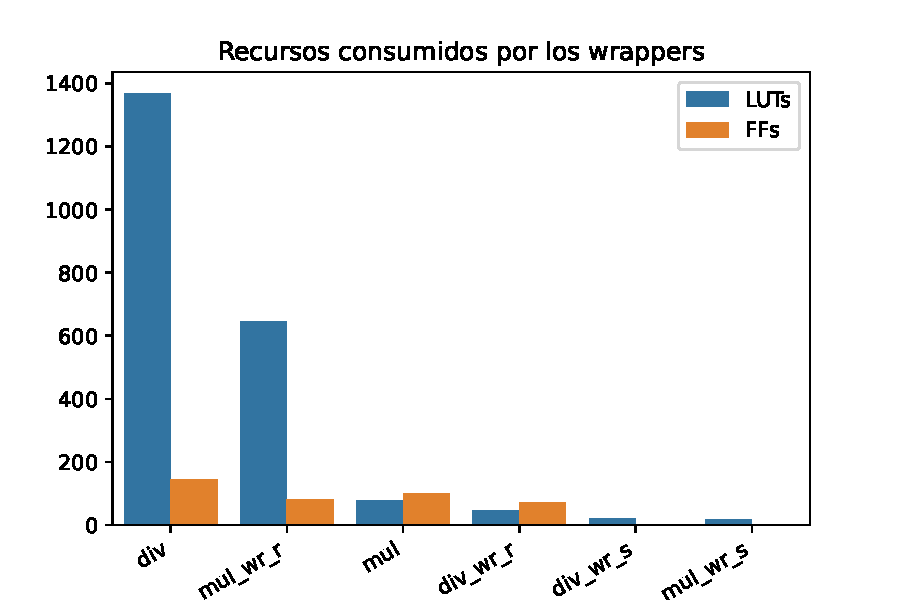
\includegraphics[width=13cm]{images/plots/swerv_wrappers.pdf}
    \caption[Recursos consumidos por los \textit{wrappers} de los submódulos de la EXU.]{Recursos consumidos por los \textit{wrappers} de los submódulos de la EXU.}
    \label{fig:plots_area_wrappers}
\end{figure}

Finalmente, analizaremos los recursos consumidos por los \textit{wrappers}, para discernir si su tamaño es debido a las unidades de cálculo (el multiplicador y el divisor en sí), o por los elementos adicionales (emisores y receptores). Se presentan una visualización de los datos en la figura \ref{fig:plots_area_wrappers}. En cuanto al divisor, su \textit{wrapper} ocupa en total 1433 LUTs, y 1368 de estos son para el submódulo divisor, por lo que los elementos adicionales de comunicación de la red emplean tan solo 65 LUTs (un 5\% del wrapper). Por otro lado, el envoltorio del multiplicador ocupa un total de 744 LUTs, mientras que su submódulo principal tan solo cuenta con 79 de estos, dejando que los dispositivos de red utilicen 665 LUTs, el 90\% del wrapper. Esto es debido a que el receptor tiene un gran tamaño, empleando 646 LUTs (86\% del wrapper).
% \tdinquiry{Ocupa un montón el receptor... ¿Eso lo digo? Tampoco sé muy bien por qué ocurre...}

Para concluir, comprobaremos qué parte de los recursos de la  EXU son consumidos por los módulos añadidos. Si sumamos los recursos consumidos por todos ellos (malla y emisores/receptores, tanto dentro como fuera de \textit{wrappers}), tenemos que se han añadido 3496LUTs y 918 FFs, principalmente debido a la malla (2700LUTs y 678FFs). Estos elementos son el 36\% de los LUTs y el 63\% de los \textit{flip-flops} de la EXU. Es decir, la inserción de la NoC ha aumentado el número de LUTs consumidos por la EXU en 57\%, y el de registros en 174\%. En conclusión, la NoC tan solo ha aumentado el tamaño total del diseño en un 9\% de LUTs y un 4\% de FFs.

% \tdinquiry[inline, caption={Cosas por hacer reportes}]{
% \begin{itemize}
%     \item Hablar de la FPGA objetivo y sus características
%     \item Área
%     \item En conclusión... las cosas añadidas suman nosecuantas LUTs y registros
% \end{itemize}
% }

